% Standalone appendix document - compiles on its own:
%   latexmk -pdf 01-project-thesis.tex
\documentclass[a4paper,11pt]{article}
\usepackage[english]{babel}
\usepackage{../../appendix-style}

\title{1.1 Project Thesis}
\author{SW4PRJ4 -- Group 3}
\date{\today}

\begin{document}
\maketitle

\begin{versionhistory}
  1.0 & 02-09-2026 & Group 3 & Initial version \\
  1.1 & 16-09-2026 & Group 3 & Rich picture, system components and sources added after review \#1 (group 4) \\
\end{versionhistory}

\section*{Problem Description}
The Danish Emergency Management Agency recommends that every Danish household keep a
supply of water, food and other essentials sufficient to cover the household for at
least three days during emergencies such as power outages, water supply failures,
severe weather or disruptions to supply chains~\cite{brs-forberedt}. The agency's
guideline is 3 litres of water per person per day and food that keeps without
refrigeration and needs no cooking~\cite{brs-forberedt}. Despite public campaigns, very
few households actually act on this. The typical barriers are:
\begin{itemize}[nosep]
  \item It is hard to work out \emph{what} and \emph{how much} one should keep in stock.
  \item The purchase has to be adapted to the size of the household and any other preferences.
  \item The household changes over time -- more or fewer residents, new preferences -- and a package that was a good fit when it was set up is not necessarily a good fit a year later.
  \item Expiry dates quietly pass, and the stock becomes outdated without anyone noticing.
  \item Having to remember to reorder manually is inconvenient.
\end{itemize}
The problem is therefore not a lack of willingness, but a lack of automation. Today
there are online shops (e.g. nemlig.com) that deliver groceries, but they offer no
coherent preparedness plan and no automatic maintenance of a personal emergency stock.

\section*{Project Description}
The project develops an \textbf{emergency preparedness subscription system} that acts as
an additional feature on top of an online grocery delivery service (simulated within the project). The system helps
households build and maintain a personal emergency stock automatically.

\subsection*{Rich Picture}
Figure~\ref{fig:rich-picture} shows the actors around the system and what flows between them.
\begin{figure}[H]
    \centering
    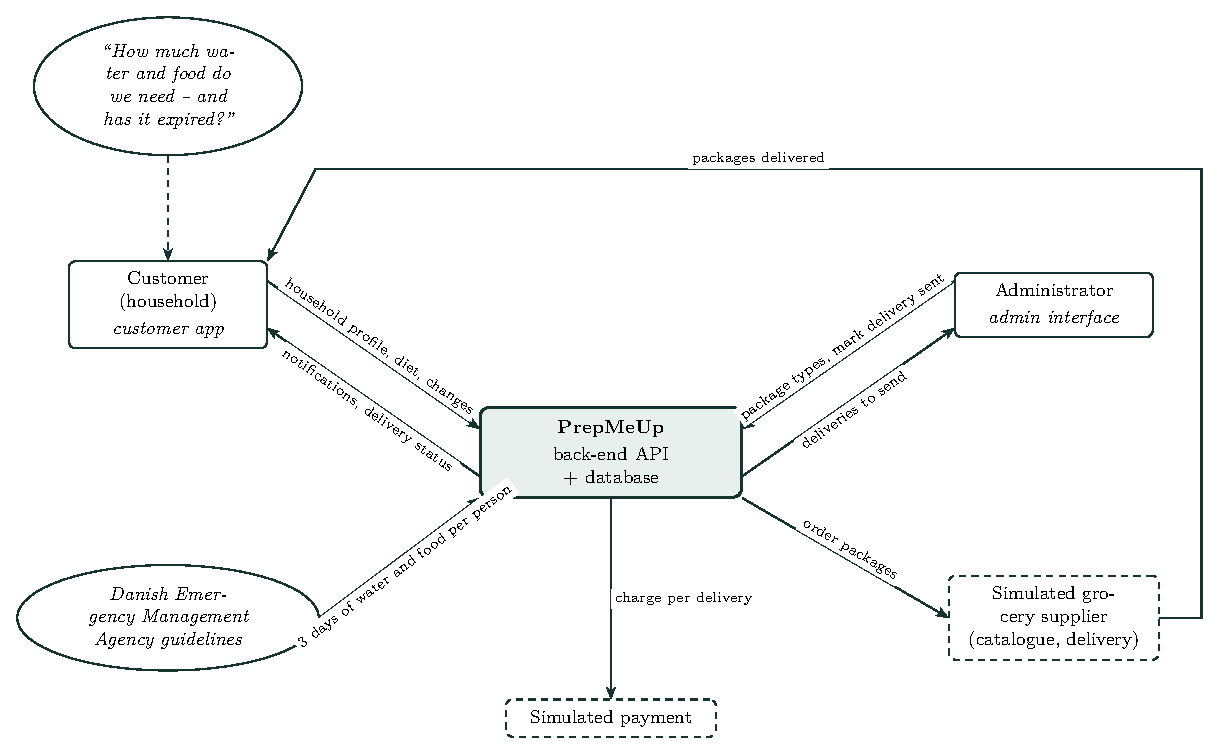
\includegraphics[width=\linewidth]{../../../assets/figures/rich-picture.pdf}
    \caption{Rich picture of PrepMeUp. Dashed boxes are simulated within the project.}
    \label{fig:rich-picture}
\end{figure}

\subsection*{System Components}
\begin{itemize}[nosep]
  \item \textbf{Customer app} (React Native, Android): sign-up, household profile, diet, delivery status and notifications.
  \item \textbf{Administrator interface} (web): maintain package types and see and dispatch upcoming deliveries.
  \item \textbf{Back-end API}: business logic -- calculates packages from the household profile, schedules reorders before expiry, sends notifications.
  \item \textbf{Database}: persistent storage of customers, households, subscriptions, deliveries and package types.
  \item \textbf{Simulated supplier and payment}: an internal service with a product catalogue and a mock delivery and card payment flow. No real supplier or payment provider is integrated.
\end{itemize}

\subsection*{Core Flow}
\begin{enumerate}[nosep]
  \item The user creates a profile describing the composition of the household (number of adults and children) along with any other preferences.
  \item The system calculates a recommended preparedness package based on the guidelines of the Danish Emergency Management Agency.
  \item The first package is delivered in one go, and the system records the expiry date of each item in the user's stock.
  \item When an item approaches its expiry date, the system schedules a reorder and sends a notification to the user.
  \item The user can adjust their profile and delivery plan based on their current stock level, pause deliveries, or mark items as ``used''.  Changes to the profile trigger a recalculation of the delivery package, so that upcoming deliveries reflect the household's current needs.
\end{enumerate}

\subsection*{Scope}
The system does not integrate with the API of an actual grocery supplier. The
``supplier'' is simulated by an internal service with a product catalogue as well as a mock
payment/delivery flow.
The system's core design covers ordinary groceries. Medicine and other prescription or regulated goods are optional expansions to the system.

\begin{thebibliography}{9}
  \bibitem{brs-forberedt} Beredskabsstyrelsen (Danish Emergency Management Agency).
  \emph{Forberedt på kriser -- sådan klarer du dig selv i tre døgn under en krise}.
  \url{https://www.brs.dk/da/forberedt/}. Accessed 16-09-2026.
\end{thebibliography}

\end{document}
